%******************************************************************************
% KOMA-Script article scrartcl
%******************************************************************************
\documentclass[11.5pt, b5paper]{article} 

% Add here all the packages that will be used in the document
%******************************************************************************
% Packages 
%******************************************************************************
% For hyperlinks 
\usepackage{url}

% Add no chapters to the article 
\usepackage[nochapters]{classicthesis}

% Setup the page geometry
\usepackage{geometry}
\geometry{a4paper, total={210mm, 297mm}, 
left=20mm, right=20mm, top=20mm, bottom=20mm}

% Use tikz to add watermarks to the document
\usepackage{blindtext,tikz}
\usetikzlibrary{calc}

% Use the classicthesis style for the style of the document
\usepackage[nochapters]{classicthesis} 

% Use the currvita style for the layout of the document
\usepackage[LabelsAligned]{currvita} 

% Required for adding links	and customizing them
\usepackage{hyperref} 

 % Set link colors
\hypersetup{colorlinks, breaklinks, urlcolor=Maroon, linkcolor=Maroon}


% Add a list of new commands 
%******************************************************************************
% Commands 
%******************************************************************************
\newcommand{\latex}{\LaTeX\xspace}
\newcommand{\tex}{\TeX\xspace}

\usepackage{listings}
\usepackage{color}
\usepackage{graphicx}
\usepackage{caption}
\usepackage{subcaption}

\graphicspath{{images/report5/}}

\definecolor{dkgreen}{rgb}{0,0.6,0}
\definecolor{gray}{rgb}{0.5,0.5,0.5}
\definecolor{mauve}{rgb}{0.58,0,0.82}

\lstset{frame=tb,
  language=Java,
  aboveskip=3mm,
  belowskip=3mm,
  showstringspaces=false,
  columns=flexible,
  basicstyle={\small\ttfamily},
  numbers=none,
  numberstyle=\tiny\color{gray},
  keywordstyle=\color{blue},
  commentstyle=\color{dkgreen},
  stringstyle=\color{mauve},
  breaklines=true,
  breakatwhitespace=true,
  tabsize=3
}

%******************************************************************************
% DOCUMENT STARTS HERE 
%******************************************************************************
\begin{document}

% TITLE 
\title{\rmfamily\normalfont\spacedallcaps{
Report \#{5}
}}

% PROJECT NAME -> ADD YOUR PROJECT NAME HERE
\author{{\small Automatic Mandible Segmentation Using VTK}}

% AUTOMATIC DATE -> DON'T CHANGE MANUALLY
\date{\footnotesize{\today}}

% MAKE THE TITLE -> DON'T CHANGE MANUALLY
\maketitle

% DON'T INCLUDE THE ABSTRACT FOR THE MOMENT
% % \begin{abstract}
% \noindent Abstract
% \end{abstract}
 
%******************************************************************************
% TABLE OF CONTENTS (uncomment to show / comment to hide)
%******************************************************************************     
% \tableofcontents


%******************************************************************************
% Report Content
%******************************************************************************
\section{Report Details}
\begin{center}
\begin{tabular}{ l | c }
\hline 
Report ID & 5   \\ % Change the sprint ID here 
\hline 
Report Duration & 1 Week \\ % Change the duration here 
\hline 
Beginning & 22.11.2016 \\ % Change the start data here
\hline 
End & 29.11.2016 \\ % Change the end data here
\hline 
\end{tabular}
\end{center}

%\section{Objectives}
\section{Original Objectives}

\section{Accomplished Objectives}

\begin{figure}
    \centering
    \begin{subfigure}[b]{0.45\textwidth}
        \centering
        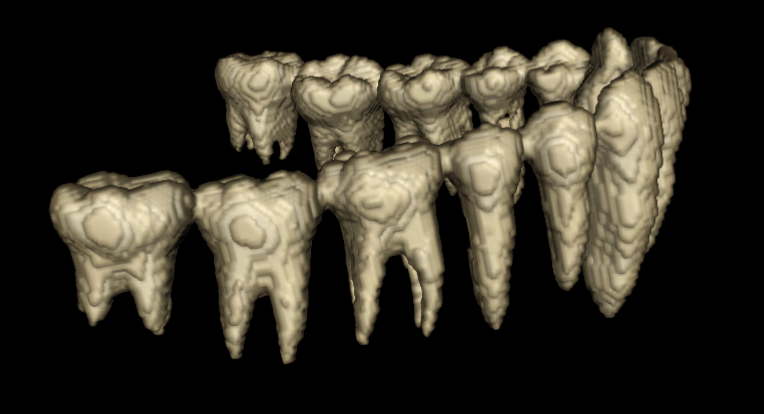
\includegraphics[width=\textwidth]{RCSO}
        \caption{Ray Casting}
    \end{subfigure}
    \hfill
    \begin{subfigure}[b]{0.45\textwidth}
        \centering
        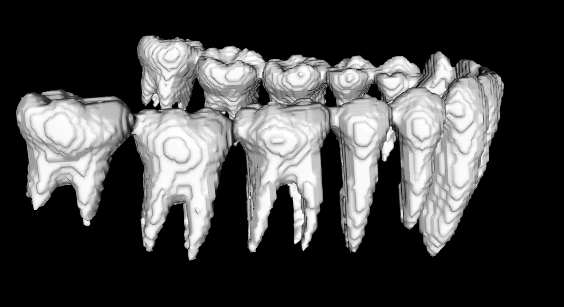
\includegraphics[width=\textwidth]{MCSO}
        \caption{Marching Cubes}
    \end{subfigure}
    \caption{Teeth Segmentation using labeling and connectivity algorithm.}
    \label{fig:CL}
\end{figure}


\begin{figure}
    \centering
    \begin{subfigure}[b]{0.5\textwidth}
        \centering
        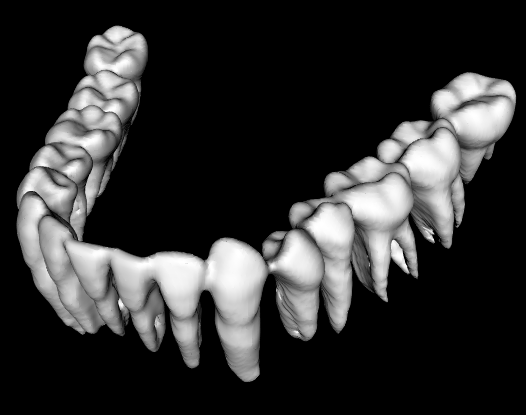
\includegraphics[width=\textwidth]{MCF1}
        \caption{Top Front View}
    \end{subfigure}
    \hfill
    \begin{subfigure}[b]{0.5\textwidth}
        \centering
        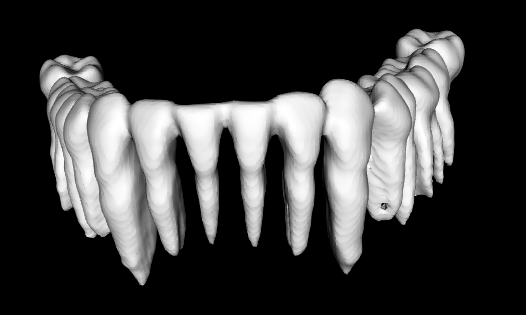
\includegraphics[width=\textwidth]{MCF2}
        \caption{Front View}
    \end{subfigure}
      \hfill
    \begin{subfigure}[b]{0.5\textwidth}
        \centering
        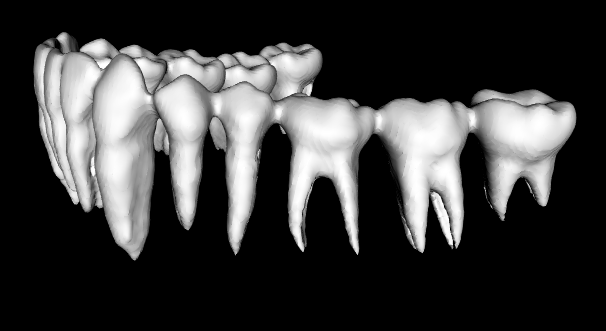
\includegraphics[width=\textwidth]{MCS1}
        \caption{First Side}
    \end{subfigure}
        \hfill
    \begin{subfigure}[b]{0.5\textwidth}
        \centering
        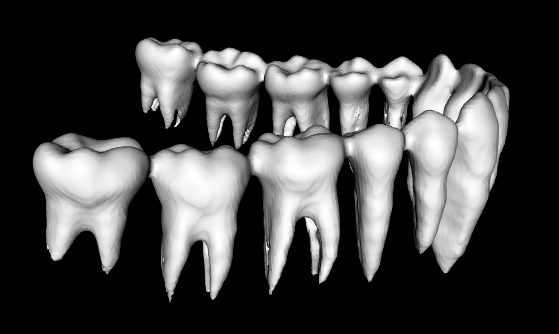
\includegraphics[width=\textwidth]{MCS2}
        \caption{Second Side}
    \end{subfigure}
    \caption{Different Views of segmented Teeth with \textit{vtkPolyDataConnectivityFilter}}
    \label{fig:PDCF}
\end{figure}

\section{Missed Objectives}

\section{Next Step}
   
%******************************************************************************
% DOCUMENT ENDS HERE 
%******************************************************************************
\end{document}